\chapter{Planejamento}
Para que todo projeto possa ser bem sucedido, devem se analisar, projetar e estudar minuciosamente e fazer o levantamento de todo os requisitos necessários para o projeto.
Apartir das matérias de Modelagem e Desenvolvimento de Sistenas e Engenharia de Software, foi possível adquirir conhecimentos para um bom planejamento do trabalho.
Como esse trabalho demonstrou ser extenso e complexo, decidimos por nos planejarmos a fim de evitar que possíveis erros de implementação fosse acarretado durante a fase de Desenvolvimento.
Assim, fizemos uma reunião inicial para decidir os pontos importantes e decidir pontos sobre implementação do código.
Utilizamos um organizador de tarefas no Excel para acompanhar as tarefas.Tal diagrama sera utilizado para as próximas etapas também.
Veja abaixo, como ficou a organização do planejamento deste trabalho na figura abaixo.

\begin{figure}[H]
    \vspace{1.0em}
    \centering
    \caption{Planejamento TP Compiladores}
    \subfloat[Diagrama Planejamento]{ % titulo da subimagem
        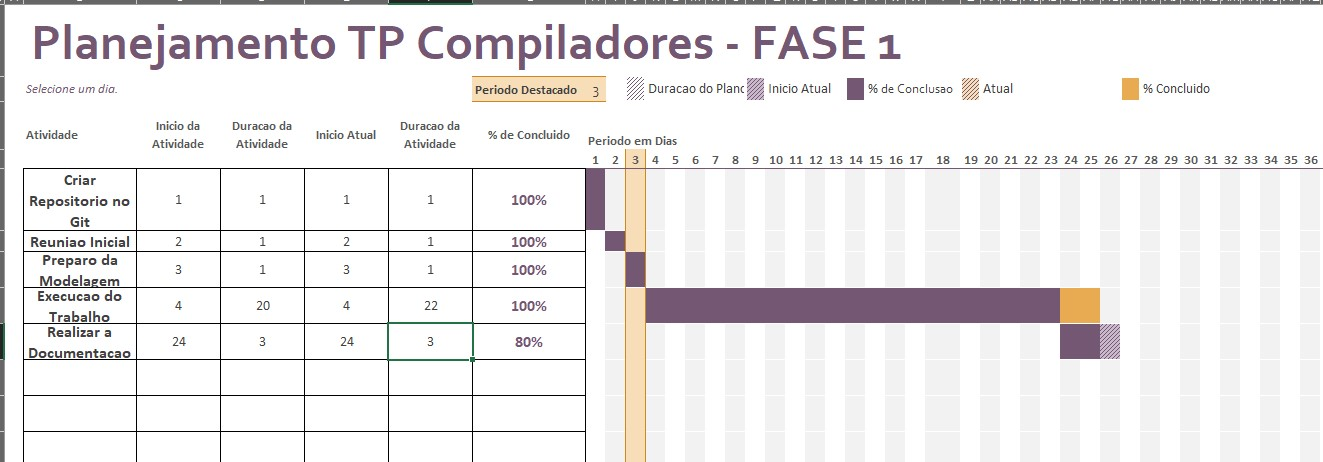
\includegraphics[width=1.0\textwidth]{img/Fase1_TpCompiladores.jpg}%
        \label{fig:pendulo_movimento}
    }
 
    \hspace{\linewidth}%
    \textbf{Fonte:} Desenvolvedores do Código
    \label{fig:cefets}
    \vspace{1.0em}
\end{figure}
Tal arquivo se encontra dentro do diretório deste projeto criado pelo Programa Microsoft Excel, podendo ser acesso pelo caminho: "TP{\_}Compilador/Planejamento/"